\documentclass{standalone}
\usepackage{pgfplots}
\pgfplotsset{compat=1.17}

\begin{document}

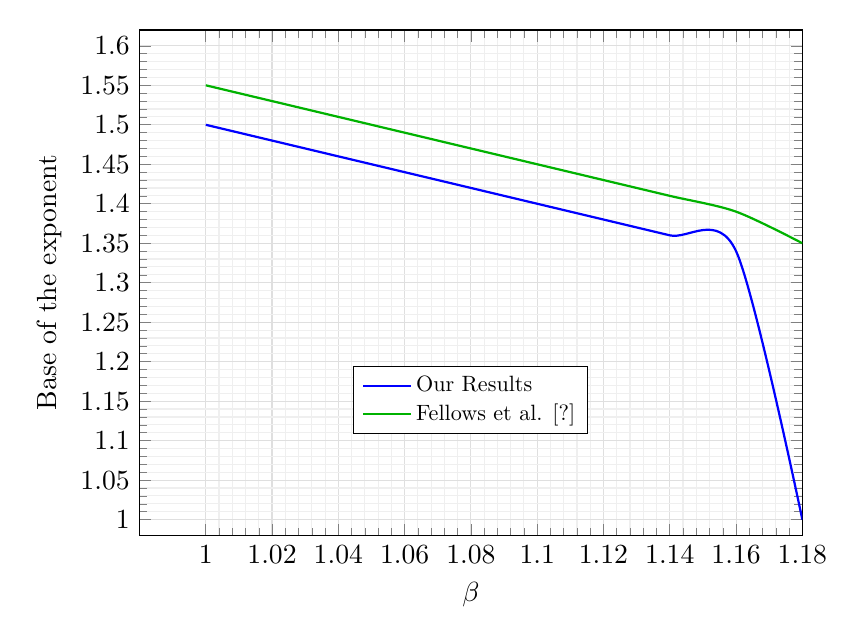
\begin{tikzpicture}
    \begin{axis}[
        xlabel={$\beta$},
        ylabel={Base of the exponent},
        xmin=0.98, xmax=1.18,
        ymin=0.98, ymax=1.62,
        xtick={1, 1.02, 1.04, 1.06, 1.08, 1.1, 1.12, 1.14, 1.16, 1.18},
        ytick={1, 1.05, 1.1, 1.15, 1.2, 1.25, 1.3, 1.35, 1.4, 1.45, 1.5, 1.55, 1.6},
        grid=both,
        minor tick num=4,
        major grid style={lightgray!50},
        minor grid style={lightgray!25},
        legend style={at={(0.5,0.2)}, anchor=south, nodes={scale=0.8, transform shape}},
        width=10cm,
        height=8cm,
        legend cell align={left},
    ]
    
    % Data points for "Our Results"
    \addplot[
        blue,
        thick,
        domain=1:1.18,
        samples=200,
        smooth,
    ] coordinates {
        (1, 1.5)
        (1.02, 1.48)
        (1.04, 1.46)
        (1.06, 1.44)
        (1.08, 1.42)
        (1.1, 1.4)
        (1.12, 1.38)
        (1.14, 1.36)
        (1.16, 1.34)
        (1.18, 1.0)
    };
    \addlegendentry{Our Results};
    
    % Data points for "Fellows et al. [?]"
    \addplot[
        green!70!black,
        thick,
        domain=1:1.18,
        samples=200,
        smooth,
    ] coordinates {
        (1, 1.55)
        (1.02, 1.53)
        (1.04, 1.51)
        (1.06, 1.49)
        (1.08, 1.47)
        (1.1, 1.45)
        (1.12, 1.43)
        (1.14, 1.41)
        (1.16, 1.39)
        (1.18, 1.35)
    };
    \addlegendentry{Fellows et al. [?]};

    \end{axis}
\end{tikzpicture}

\end{document}